\begin{frame}{A General Model of Repeated Games}
    \tikzstyle{every picture}+=[remember picture]
    \tikzstyle{na} = [baseline=-.5ex]

    \begin{equation*}
        \Gamma^r =
            \only<1>{(
                N, \Theta, (D_i, S_i, u_i)_{i\in N}, q, p)
            }
            \only<2>{(
                \tikz[baseline]{
                    \node[fill=green!20, ellipse, anchor=base] (t1) {$N$};
                }, \Theta, (D_i, S_i, u_i)_{i\in N}, q, p)
            }
            \only<3>{(N, 
                \tikz[baseline]{
                    \node[fill=green!20, ellipse, anchor=base] (t1) {$\Theta$};
                }, (D_i, S_i, u_i)_{i\in N}, q, p)
            }
            \only<4>{(N, \Theta, (
                \tikz[baseline]{
                    \node[fill=green!20, ellipse, anchor=base] (t1) {$D_i$};
                }, S_i, u_i)_{i\in N}, q, p)
            }
            \only<5>{(N, \Theta, (D_i,
                \tikz[baseline]{
                    \node[fill=green!20, ellipse, anchor=base] (t1) {$S_i$};
                }, u_i)_{i\in N}, q, p)
            }
            \only<6>{(N, \Theta, (D_i, S_i,
                \tikz[baseline]{
                    \node[fill=green!20, ellipse, anchor=base] (t1) {$u_i$};
                })_{i\in N}, q, p)
            }
            \only<7>{(N, \Theta, (D_i, S_i, u_i)_{i\in N},
                \tikz[baseline]{
                    \node[fill=green!20, ellipse, anchor=base] (t1) {$q$};
                }, p)
            }
            \only<8>{(N, \Theta, (D_i, S_i, u_i)_{i\in N}, q,
                \tikz[baseline]{
                    \node[fill=green!20, ellipse, anchor=base] (t1) {$p$};
                })
            }
    \end{equation*}

    \begin{itemize}[<+->]
        \pause
        \item {\color<2>{green} Non-empty set of players}
        \item {\color<3>{green} Non-empty set of possible states of nature}
        \item {\color<4>{green} Set of moves player $i$ can choose at each round of the game. Let
        \[ D = \bigtimes_{i\in N} D_i .\]}
        \item {\color<5>{green} Set of signals player $i$ can receiver each round of the game. Let
        \[ S = \bigtimes_{i\in N} S_i .\]}
        \item {\color<6>{green} $u_i: D\times \Theta \to \mathbb{R}$ is the payoff function of player $i$}
        \item {\color<7>{green} $q \in \Delta(S \times \Theta)$ is the initial distribution}
        \item {\color<8>{green} $p: D\times \Theta \to \Delta(S \times \Theta)$ is the transition function}
    \end{itemize}
\end{frame}

\note{
    Model for the repeated Prisoner's Dilemma on the blackboard
    \begin{itemize}
        \item $N = \{1, 2\}$
        \item $\Theta = \{\text{active}, \text{stopped}\}$
        \item $D_1 = \{C, D\}$, $D_2 = \{c, d\}$ and $D = D_1 \times D_2$
        \item $S_i = \Theta \cup (D_1 \times D_2) = \{\text{active}, \text{stopped}, Cc, Cd, Dc, Dd\}$
        and $S = S_1 \times S_2$
        \item $u_i(d, \text{active})$ corresponds to the payoffs indicated in the normal form of the game while
        $u_i(d, \text{active}) = 0$, $\forall d \in D$
        \item $q\left((\text{active}, \text{active}), \text{active}\right) = 1$
        \item $p\left((d, d), \text{active}~|~ d, \text{active}\right) = 5/6$, 
        $p\left((\text{stopped}, \text{stopped}), \text{stopped}~|~ d, \text{active}\right)  = 1/6$ and
        $p\left((\text{stopped}, \text{stopped}), \text{stopped}~|~ d, \text{stopped}\right)  = 1$
        $\forall d \in D$
    \end{itemize}
}

\begin{frame}{Stochastic Game visualized}
    \begin{figure}
        \centering
        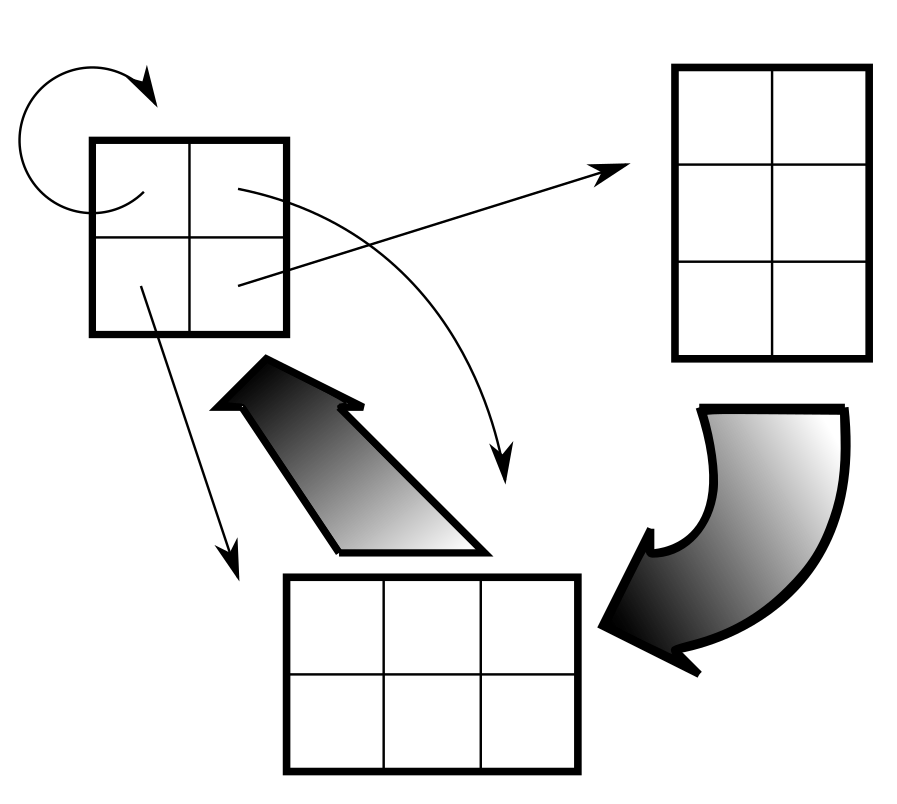
\includegraphics[width=0.6\textwidth]{img/stochastic.png}
        \caption{An illustration of what a Stochastic Game is. \\
        \small{Taken from ``Game Theory'' I on Coursera, by Jackson, Leyton-Brown \& Shoham.}}
    \end{figure}
\end{frame}

\note{
    \begin{itemize}
        \item agents repeatedly play games from a set of different games,
        \item the game played at each round depends on the previous game played and the
        actions taken by each players in that game.
    \end{itemize}
}

\begin{frame}{Pure strategies in infinitely repeated games}
    \begin{block}{How do we define pure strategies from that model?}
        \begin{itemize}[<+->]
            \item In a general repeated game, we assume that each player at each round $k$ recalls
            all the signals that he has gotten in rounds 1 through $k$.
            \item The set of all possible such \textit{histories of signals} for player $i$ is given by the
            $k$-fold Cartesian product of $S_i$
            \[ (S_i)^k = \underbrace{S_i \times \dots \times S_i}_{k\text{ times}}.\]
            \item A pure strategy for round $k$ is a map between each possible history in $(S_i)^k$
            and a move in $D_i$
            \[ c^k_i: (S_i)^k \to D_i. \]
            \item The set of all pure strategies for player $i$ is
            \[ C_i = \{c_i = (c_i^k)_{k=1}^\infty~|~ c_i^k: (S_i)^k \to D_i \}. \]
        \end{itemize}
    \end{block}
\end{frame}

\begin{frame}{Behavioral strategies in infinitely repeated games}
    \begin{block}{And for behavioral strategies?}
        In the same manner, the set of all behavioral strategies for player $i$ is
        \[ B_i = \{\sigma_i = (\sigma_i^k)_{k=1}^\infty~|~ \sigma_i^k: (S_i)^k
        \to {\color{green}\Delta}(D_i) \}. \]
    \end{block}
\end{frame}

\begin{frame}{Equilibrium}
    \begin{block}{Equilibrium}
        By defining some additionial quantities and doing some more {\color{orange}cumbersome}
        math, we can define what an \textit{equilibrium} is (for the different criteria for
        ranking payoffs given in the previous section).
    \end{block}

    \begin{alertblock}{Challenges}
        Because the set of behavioral strategies is \textbf{infinite}, checking if a strategy is an
        equilibrium is very hard.
    \end{alertblock}
\end{frame}

\note{
    We should briefly explain why the set of behavioral strategy is infinite here.
}

\begin{frame}{The bounded rationality principle to the rescue}
    \begin{exampleblock}{The bounded rationality principle}
        In practice, we can limit the history of past signals received to the $l$ last signals
        to define strategies.\\
        {\color{green}$\to$ the set of behavioral strategies is now finite!}
    \end{exampleblock}

    \vspace{0.5cm}
    \begin{block}{One possible interpretation}
        We can think of that as a rational players programming a computer with limited memory and
        computational power to choose its moves.
    \end{block}
\end{frame}

\begin{frame}{A Taxonomy of Repeated Games Models}
    \begin{figure}
        \tikzstyle{mybox} = [draw=gray!20, fill=white, very thick,
        rectangle, rounded corners, inner sep=10pt, inner ysep=10pt]
        \tikzstyle{fancytitle} = [fill=gray, text=white, rounded corners]
        \scalebox{0.7}{
        \begin{tikzpicture}
            \node [mybox, draw=black] at (0, 0) (gen-mod){%
                \begin{minipage}{0.50\textwidth}
                    \vspace{-0.25cm}
                    \[ \Gamma^r = (N, \Theta, (D_i, S_i, u_i)_{i\in N}, q, p) \]
                \end{minipage}
            };
            \node [inner sep=0pt] (gen-mod-img) at (-4.4, 0.5){%
                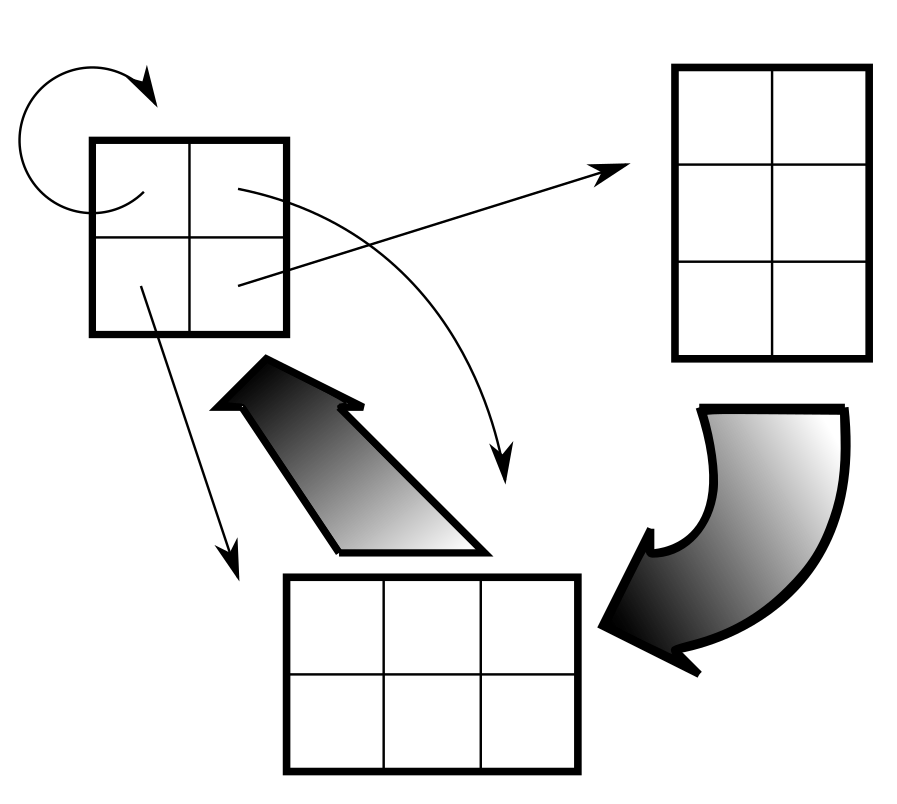
\includegraphics[width=0.25\textwidth]{img/stochastic.png}
            };
            
            \node [mybox] at (-4.5, -3) (mdp){%
                \begin{minipage}{0.40\textwidth}
                    {\color{green}Single-agent stochastic game}
                    \vspace{-0.25cm}
                    \[ |N| = 1. \]
                \end{minipage}
            };
            
            \node [mybox] at (0, -7.5) (state){%
                \begin{minipage}{\textwidth}
                    {\color{green}At every round, every player knows the
                    current state of nature $\theta \in \Theta$.} \\
                    Informally, for each player $i \in N$, there exists some
                    state $w(s_i) \in \Theta$ such that the signal $s_i$ can
                    never occur unless the current state is $w(s_i)$.
                \end{minipage}
            };
            
            \node [mybox] at (4.5, -3.5) (std){%
                \begin{minipage}{0.60\textwidth}
                    \begin{itemize}
                        \item {\color{green}Only one possible state of
                        nature}
                        \[ |\Theta| = 1. \]
                        \item {\color{green}Players know all of each other's past
                        moves}
                        \[ S_i = \bigtimes_{j\in N-i} D_j. \]
                    \end{itemize}
                \end{minipage}
            };
            \node [inner sep=0pt] (gen-mod-img) at (7, -5.5){%
                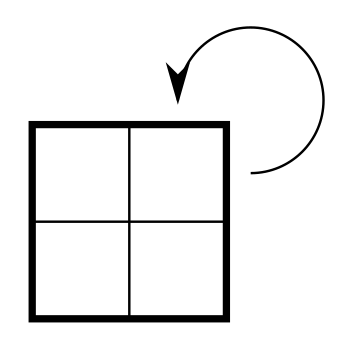
\includegraphics[width=0.20\textwidth]{img/std.png}
            };

            \node[fancytitle, fill=black] at (gen-mod.north) {Stochastic Games (General Model)};
            \node[fancytitle] at (mdp.north) (mdp-title) {Markov Decision Processes};
            \node[fancytitle] at (state.north) (state-title) {Complete State Information};
            \node[fancytitle] at (std.north) (std-title) {Standard Repeated Games};

            \draw[thick, -Latex] (gen-mod.west) -- (mdp-title.north);
            \draw[thick, -Latex] (gen-mod.south) -- (state-title.north);
            \draw[thick, -Latex] (gen-mod.east) -- (std-title.north);
        \end{tikzpicture}}
        \caption{A taxonomy of repeated game models.}
    \end{figure}
\end{frame}

\note{
    The model we just derived is the one highlighted in black.

    Explain that it generalizes Markov Decision Processes (MDPs).

    Recall the plan for the rest of the presentation by showing the two other
    models on this diagram.
}

\begin{frame}{Take-home message \#4}
    \todo[inline]{I still need to find a short enough message for this section.}
\end{frame}
